\chapter{関連研究}
\label{chp:first}

\section{関連研究}
\label{sec:paragraph}

新しいマテリアルを使い,今までにない3Dプリンターでは表現できなかったモノを作ることを可能にしている研究を中心最新の3Dプリンターに関する研究を調査した.


\section{ゲルを用いて印刷する3Dプリンター}
\label{sec:enum}

この研究は,ゲルをマテリアルとして用いた造形物を3Dプリンディングするものである.
図1のように,ゲル溶液を使用しながら強度や感触を部位によって変化させて造形物を作成することができる.

\begin{figure}[H]
  \centering
  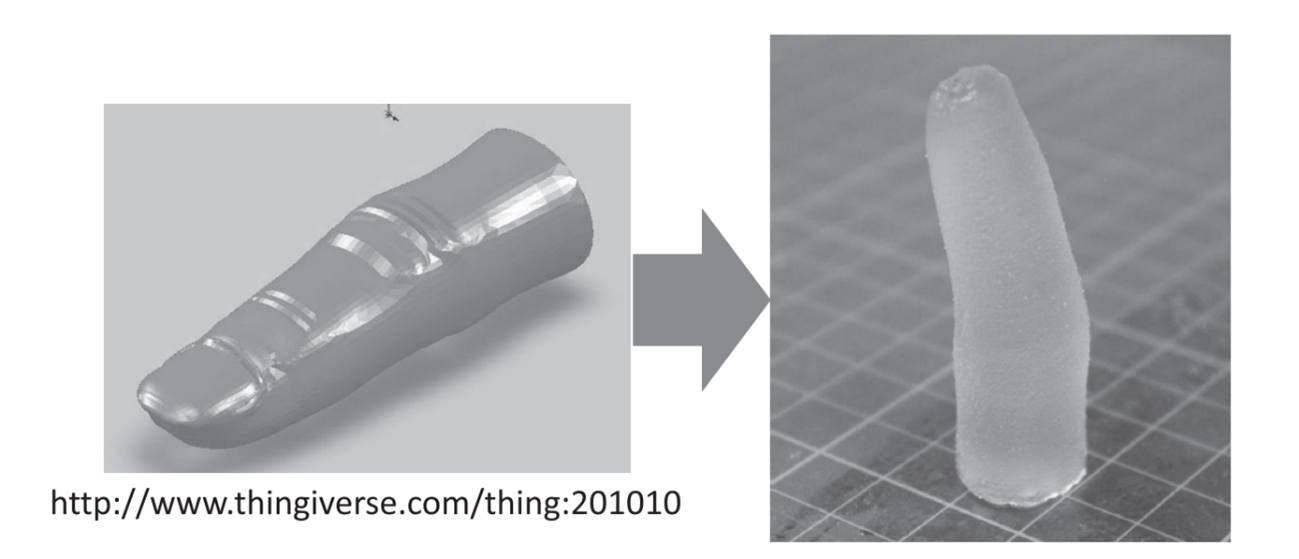
\includegraphics[width=6.4truecm]{./fig/ゲルを用いて印刷する3Dプリンター.png}
  \caption{適当なサンプル2}
% \url{http://www.this.is.sample.url/} % Web上のデータの場合、参照先URLを明記
  \label{fig:ferret}
\end{figure}

これは,ゲル化を誘起するUVレーザーを光ファイバーを通して局所的にゲル溶液に照射することで,ゲルの3次元造形を可能にしている.3Dプリンターは現在,臓器の立体イメージを作り出すのに医療分野で活用されているが,手術の計画や事前検証のための立体の臓器モデルを作製するには,数千万もする工学な3Dプリンターを使用してプラスチックやゴムなどの,実際の臓器よりもはるかに硬い樹脂を用いて造形をする方法しか存在しなかった.
このゲルを用いて印刷する3Dプリンターは,低コストで感触がより患者のものと似ている臓器モデルを作成できる可能性を秘めている.

この3Dプリンターは材料として微粒子調整ダブルネットワークゲル(略称:P-DNゲル)を使用している.このゲルは強電解質性を示すモノマー由来の堅く脆い高分子ネットワーク(1st ネットワーク)と,中性を示すモノマー由来の柔軟な高分子ネットワーク(2nd ネットワーク)が相互侵入網目構造をとっている複合材料である.このP-DNゲル溶液にUVレーザーを照射することでラジカル反応が生じ,ゲルの3次元構造をつくることができる.


\section{Suntory-3D on the Rocks}
\label{sec:enum}

氷を掘削し様々な彫刻を作りお酒に入れて楽しむ試みがある.
多軸の CNC を使い掘削することで高精度の彫刻を作ることができるが,一般に普及させるのはコストならびに加工中の冷却の面から考えると難しい.

\begin{figure}[H]
  \centering
  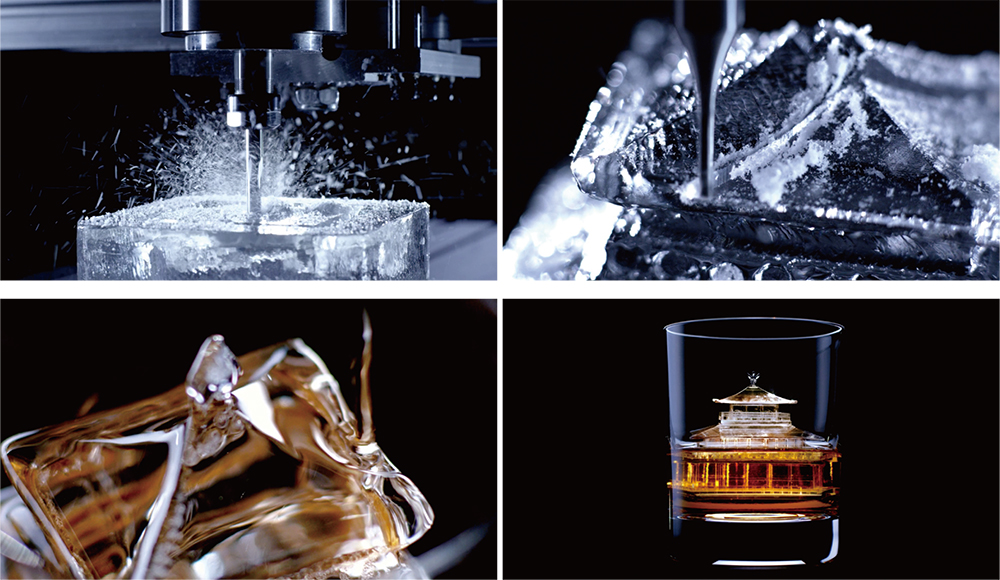
\includegraphics[width=6.4truecm]{./fig/Suntory-3D on the Rocks.jpg}
  \caption{適当なサンプル2}
% \url{http://www.this.is.sample.url/} % Web上のデータの場合、参照先URLを明記
  \label{fig:ferret}
\end{figure}


\section{Robot-Assisted Rapid Prototyping for Ice Structures}
 \label{sec:enum}
この研究では,冷やした水を一滴ずつ垂らしながら氷をFDM の様に積み上げて造形する.
造形のスピードはかなり遅く 20mm/h で造形するが,精密な造形が可能で塩水をサポート剤として使用し,オーバーハングのある造形も可能になっている.
塩水でできた氷は水でできた氷よりも低い温度で溶け始めるため.0 度の部屋で放置すれば塩水のラフトが溶け水の造形物だけが残る仕組みになっている.
過去にも水を垂らしながら造形する研究があり,-20° Cの水を液体の状態を保つために急速冷凍を防止する研究を参考にしている.
この研究は精度を出すためにスピードを犠牲にしており普通のマグカップのサイズでも印刷に 50時間近くかかる.そのため,造形中に溶けないように冷凍庫の中のような環境の部屋で造形する必要がある.
\begin{figure}[H]
  \centering
  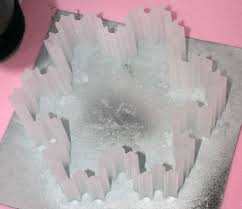
\includegraphics[width=6.4truecm]{./fig/Robot-Assisted Rapid Prototyping for Ice Structures.png}
  \caption{適当なサンプル2}
% \url{http://www.this.is.sample.url/} % Web上のデータの場合、参照先URLを明記
  \label{fig:ferret}
\end{figure}
